\section{Application Tracing}

\begin{frame}[fragile]
  \frametitle{strace}
  \begin{columns}
  \column{0.75\textwidth}
  \small
  System call tracer - \url{https://strace.io}
  \begin{itemize}
  \item Available on all GNU/Linux systems\\
        Can be built by your cross-compiling toolchain generator or by your build system.
  \item Allows to see what any of your processes is doing: accessing files, allocating memory...
        Often sufficient to find simple bugs.
  \item Usage:\\
    \code{strace <command>} (starting a new process)\\
    \code{strace -p <pid>} (tracing an existing process)\\
    \code{strace -c <command>} (statistics of system calls taking most time)
  \end{itemize}
  See \href{https://man7.org/linux/man-pages/man1/strace.1.html}{the strace manual} for details.
  \column{0.25\textwidth}
  \includegraphics[height=0.7\textheight]{common/strace-mascot.png}\\
  \tiny Image credits: \url{https://strace.io/}
  \end{columns}
\end{frame}

\begin{frame}[fragile]
  \frametitle{strace example output}
  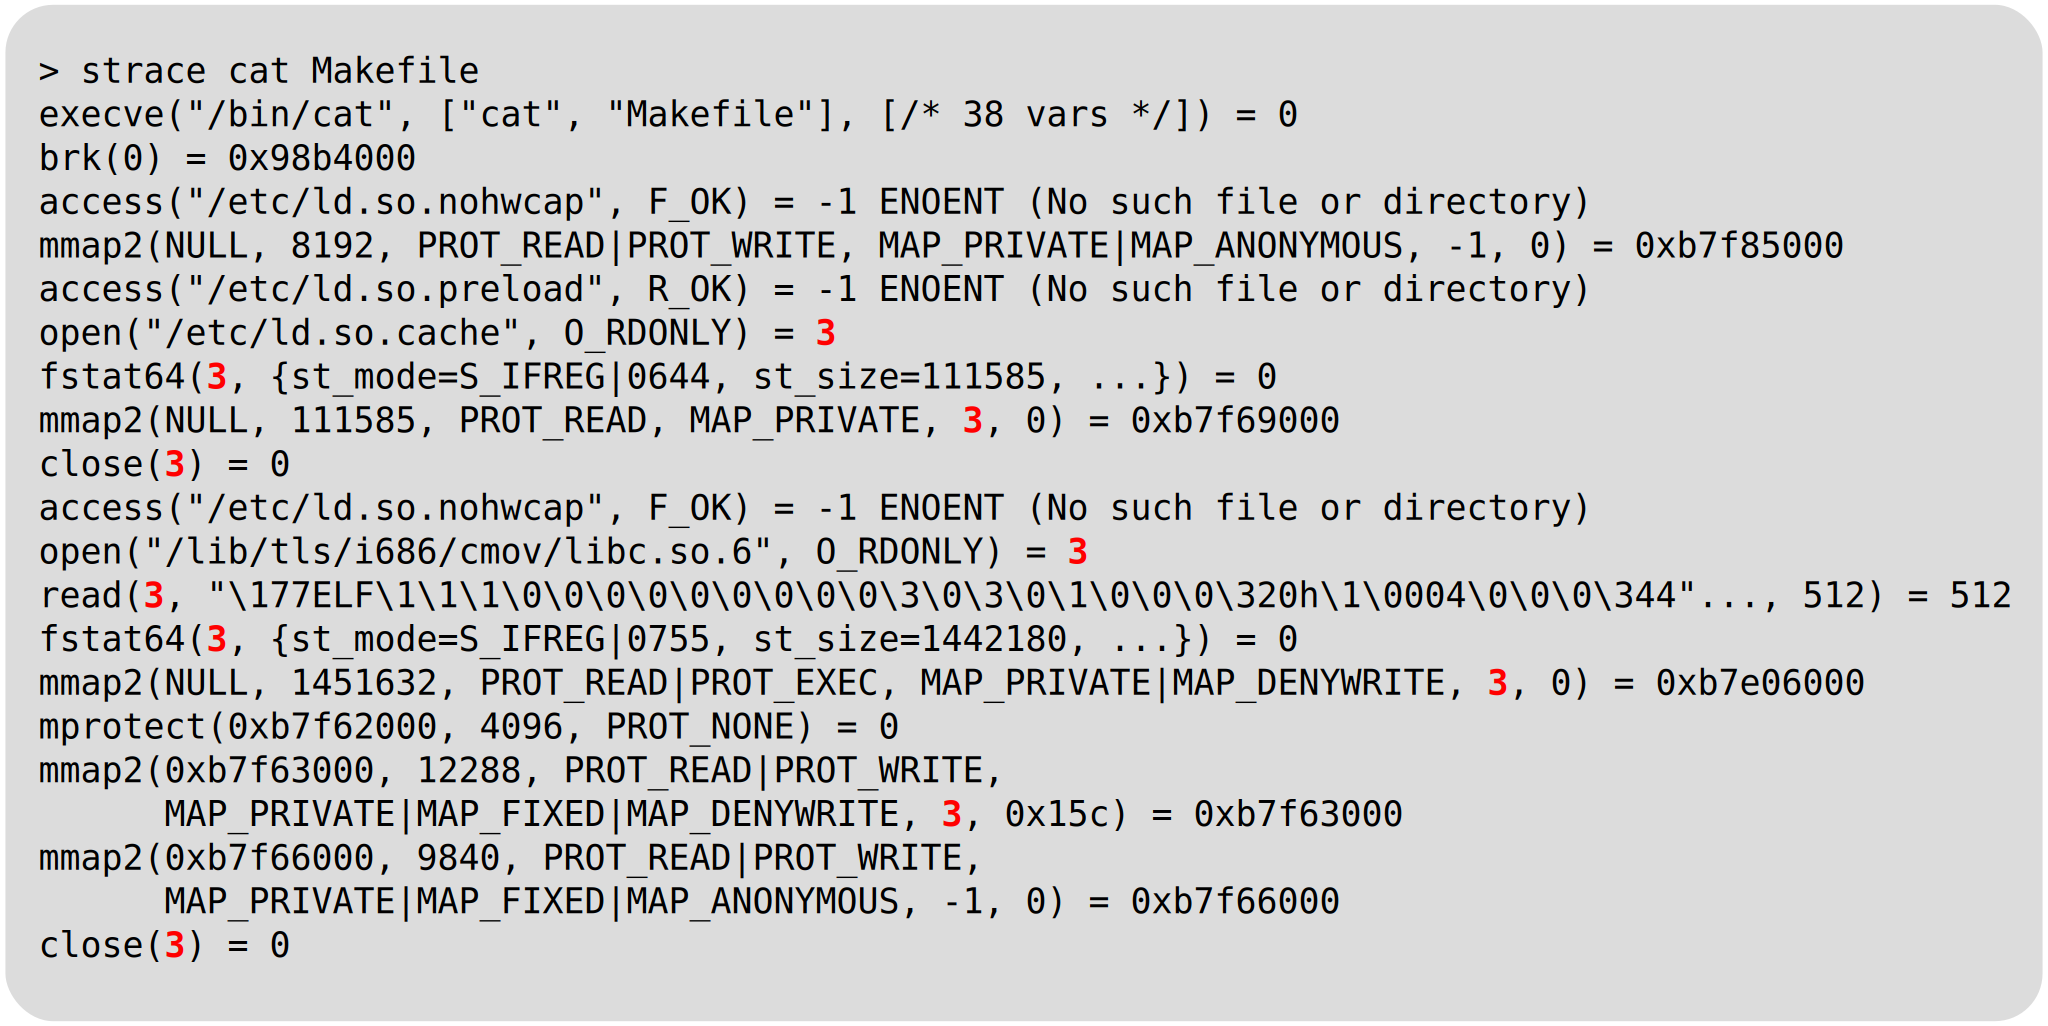
\includegraphics[height=0.75\textheight]{common/strace-output.pdf}\\
  Hint: follow the open file descriptors returned by \code{open()}.
  This tells you what files are handled by further system calls.
\end{frame}

\begin{frame}[fragile]
  \frametitle{strace -c example output}
  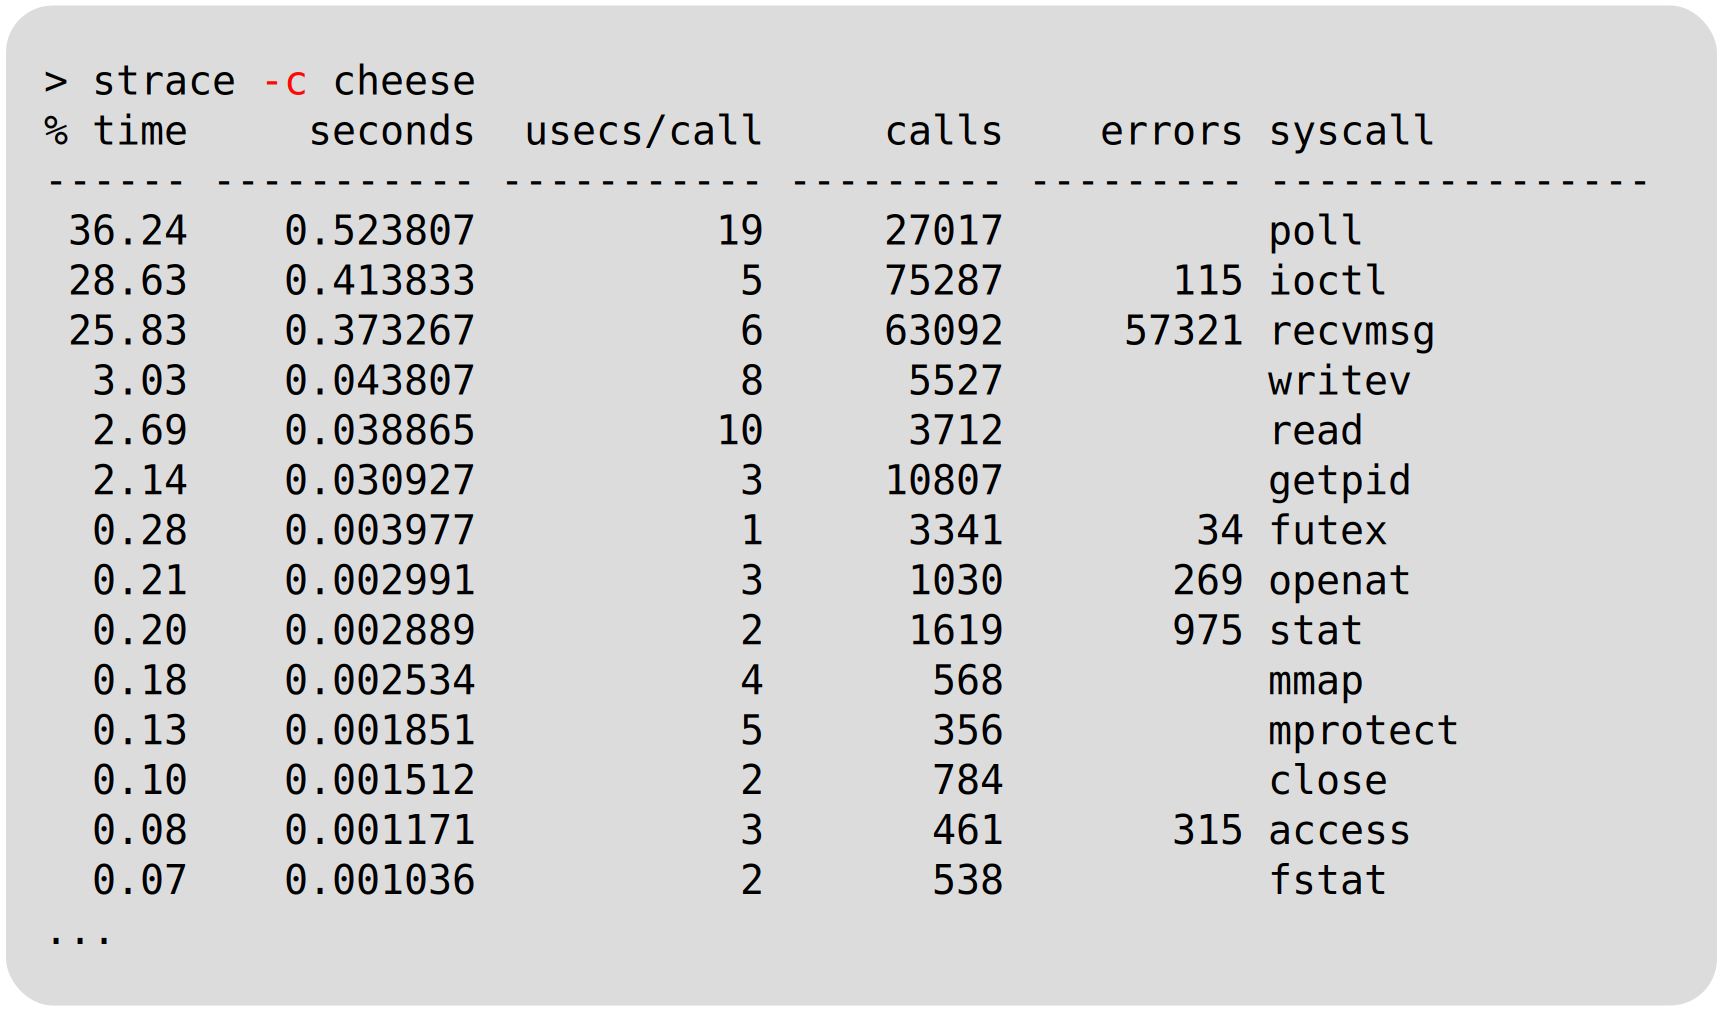
\includegraphics[height=0.8\textheight]{common/strace-c-output.pdf}
\end{frame}

\begin{frame}
  \frametitle{ltrace}
  A tool to trace library calls used by a program and all the signals
  it receives
  \begin{itemize}
  \item Very useful complement to \code{strace}, which shows only system
    calls. Library calls include system calls too!
  \item Of course, works even if you don't have the sources
  \item Allows to filter library calls with regular expressions, or
    just by a list of function names.
  \item Also offers a summary with its \code{-c} option.
  \item Manual page: \url{https://linux.die.net/man/1/ltrace}
  \item Works better with {\em glibc}. \code{ltrace} was broken
        with {\em uClibc} and may still be.
  \end{itemize}
  See \url{https://en.wikipedia.org/wiki/Ltrace} for details
\end{frame}

\begin{frame}[fragile]
  \frametitle{ltrace example output}
  \small
  \begin{block}{}
\begin{verbatim}
ltrace nedit index.html
sscanf(0x8274af1, 0x8132618, 0x8248640, 0xbfaadfe8, 0) = 1
sprintf("const 0", "const %d", 0) = 7
strcmp("startScan", "const 0") = 1
strcmp("ScanDistance", "const 0") = -1
strcmp("const 200", "const 0") = 1
strcmp("$list_dialog_button", "const 0") = -1
strcmp("$shell_cmd_status", "const 0") = -1
strcmp("$read_status", "const 0") = -1
strcmp("$search_end", "const 0") = -1
strcmp("$string_dialog_button", "const 0") = -1
strcmp("$rangeset_list", "const 0") = -1
strcmp("$calltip_ID", "const 0") = -1
\end{verbatim}
\end{block}
\end{frame}


\begin{frame}
  \frametitle{Hooking Library Calls}
  \begin{itemize}
    \item In order to do some more complex library call hooks, one can use
          the {\em LD\_PRELOAD} environment variable.
    \item {\em LD\_PRELOAD} is used to specify a shared library that will be
          loaded before any other library by the dynamic loader.
    \item Allows to intercept all library calls by preloading another library.
    \begin{itemize}
      \item Overrides libraries symbols that have the same name.
      \item Allows to redefine only a few specific symbols.
      \item "Real" symbol can still be loaded and used with \code{dlsym} (\manpage{dlsym}{3})
    \end{itemize}
    \item Used by some debugging/tracing libraries ({\em libsegfault},
          {\em libefence})
    \item Works for C and C++.
  \end{itemize}
\end{frame}

\begin{frame}[fragile]
  \frametitle{{\em LD\_PRELOAD} example}
  \begin{itemize}
    \item Library snippet that we want to preload using {\em LD\_PRELOAD}:
  \end{itemize}
  \begin{block}{}
    \begin{minted}[fontsize=\small]{c}
#include <string.h>
#include <unistd.h>

ssize_t read(int fd, void *data, size_t size) {
  memset(data, 0x42, size);
  return size;
}
    \end{minted}
  \end{block}
  \begin{itemize}
    \item Compilation of the library for {\em LD\_PRELOAD} usage:
  \end{itemize}
  \begin{block}{}
    \begin{minted}[fontsize=\small]{console}
$ gcc -shared -fPIC -o my_lib.so my_lib.c
    \end{minted}
  \end{block}

  \begin{itemize}
    \item Preloading the new library using {\em LD\_PRELOAD}:
  \end{itemize}
  \begin{block}{}
    \begin{minted}[fontsize=\small]{console}
$ LD_PRELOAD=./my_lib.so ./exe
    \end{minted}
  \end{block}
\end{frame}

\begin{frame}[fragile]
  \frametitle{uprobes}
  \begin{itemize}
    \item {\em uprobe} is a mechanism offered by the kernel allowing to trace
          userspace code.
    \item Tracepoints can be added dynamically on any userspace symbol
    \begin{itemize}
      \item Internally patches the \code{.text} section with breakpoints
        that are handled by the kernel trace system
    \end{itemize}
    \item Exposed by file \code{/sys/kernel/debug/tracing/uprobe_events}
    \item Often wrapped up by other tools (\code{perf}, \code{bcc} for
          instance).
    \item \kdochtml{trace/uprobetracer}
  \end{itemize}
\end{frame}

\begin{frame}[fragile]
  \frametitle{The {\em perf} tool}
  \begin{itemize}
    \item {\em perf} tool was started as a tool to profile application under
          Linux using performance counters (\manpage{perf}{1}).
    \item It became much more than that and now allows to manage tracepoints,
          kprobes and uprobes.
    \item {\em perf} can profile both user-space and kernel-space execution.
    \item {\em perf} is based on the \code{perf_event} interface that is
          exposed by the kernel.
    \item Provides a set of operations, each having specific arguments (see
          {\em perf} help).
    \begin{itemize}
      \item \code{stat}, \code{record}, \code{report}, \code{top}, \code{annotate}, \code{ftrace}, \code{list}, \code{probe}, etc
    \end{itemize}
  \end{itemize}
\end{frame}

\begin{frame}[fragile]
  \frametitle{Using {\em perf record}}
  \begin{itemize}
    \item {\em perf record} allows to record performance events per-thread,
          per-process and per-cpu basis.
    \item Kernel needs to be configured with \kconfigval{CONFIG_PERF_EVENTS}{y}.
    \item This is the first command that needs to be run to gather data from
          program execution and output them into \code{perf.data}.
    \item \code{perf.data} file can then be analyzed using \code{perf annotate}
          and \code{perf report}.
    \begin{itemize}
      \item Useful on embedded systems to analyze data on another computer.
    \end{itemize}
  \end{itemize}
\end{frame}

\begin{frame}[fragile]
  \frametitle{Probing userspace functions}
  \begin{itemize}
    \item List functions that can be probed in a specific
          executable:
  \begin{block}{}
    \begin{minted}[fontsize=\scriptsize]{C}
$ perf probe --source=<source_dir> -x my_app -F
    \end{minted}
  \end{block}
    \item List lines number that can be probed in a specific
          executable/function:
  \begin{block}{}
    \begin{minted}[fontsize=\scriptsize]{C}
$ perf probe --source=<source_dir> -x my_app -L my_func
    \end{minted}
  \end{block}
    \item Create tracepoints on user-space library/executable functions:
  \begin{block}{}
    \begin{minted}[fontsize=\scriptsize]{C}
$ perf probe -x /lib/libc.so.6 printf
$ perf probe -x app my_func:3 my_var
$ perf probe -x app my_func%return ret=%r0
    \end{minted}
  \end{block}
  \item Record the execution of these tracepoints:
  \begin{block}{}
    \begin{minted}[fontsize=\scriptsize]{C}
$ perf record -e probe_app:my_func -e probe_libc:printf
    \end{minted}
  \end{block}
  \end{itemize}
\end{frame}

\setuplabframe
{Application tracing}
{
  Analyzing of application interactions
  \begin{itemize}
    \item Analyze dynamic library calls from an application using
            {\em ltrace}.
    \item Using {\em strace} to analyze program syscalls.
  \end{itemize}
}
